% !TeX program = lualatex
\documentclass[aspectratio=169,11pt]{beamer}
\usepackage{amsmath,amssymb,tikz,array}
\usetikzlibrary{arrows.meta,positioning}
\useoutertheme{miniframes}

% Match Lecture09.pdf: Computer Modern, NYU purple, narrow margins,
% section navigation, two-line footer, and lightly outlined proof states.
\definecolor{nyu}{HTML}{57068C}
\definecolor{navpurple}{HTML}{4C2A7E}
\setbeamercolor{structure}{fg=nyu}
\setbeamercolor{frametitle}{fg=nyu,bg=white}
\setbeamercolor{section in head/foot}{fg=white,bg=navpurple}
\setbeamercolor{author in head/foot}{fg=white,bg=navpurple}
\setbeamercolor{title in head/foot}{fg=white,bg=navpurple!92!black}
\setbeamercolor{normal text}{fg=black,bg=white}
\setbeamertemplate{navigation symbols}{}
\setbeamertemplate{mini frames}[default]
\setbeamersize{text margin left=3mm,text margin right=3mm}
\setbeamerfont{frametitle}{size=\large}
\setbeamerfont{section in head/foot}{size=\fontsize{6}{7}\selectfont,series=\mdseries}
\setbeamerfont{author in head/foot}{size=\fontsize{6}{7}\selectfont,series=\mdseries}
\setbeamerfont{title in head/foot}{size=\fontsize{6}{7}\selectfont,series=\mdseries}
\setbeamertemplate{footline}{%
  \begin{beamercolorbox}[wd=\paperwidth,ht=2.4mm,dp=1mm,leftskip=3mm,rightskip=3mm]{author in head/foot}%
    \usebeamerfont{author in head/foot}Jaume\hfill NYU
  \end{beamercolorbox}%
  \begin{beamercolorbox}[wd=\paperwidth,ht=2.4mm,dp=1mm,leftskip=3mm,rightskip=3mm]{title in head/foot}%
    \usebeamerfont{title in head/foot}Week 11: SOS and proofs by reflection\hfill\insertframenumber/\inserttotalframenumber
  \end{beamercolorbox}%
}
\title{Proofs and computation}
\subtitle{\normalsize
  (1) Proofs by verifying external computations.\\[3mm]
  (2) Proofs by verifying an external checker.}
\author{Jaume de Dios Pont}
\institute{New York University}
\date{November 18, 2026}
\hypersetup{pdftitle={Week 11: SOS and proofs by reflection},pdfauthor={Jaume de Dios Pont}}

\newcommand{\code}[1]{\texttt{#1}}
\tikzset{
  proof/.style={draw=nyu!25,fill=nyu!2,inner sep=7pt,align=left},
  flow/.style={draw=black!42,semithick,-{Stealth[length=3pt,width=4pt]}},
  labeltext/.style={font=\small,text=black!65,align=center},
  purple/.style={text=nyu},
}

\begin{document}
% !TeX root = Lecture11.tex
% Content and instructor notes. Style is in Lecture11.tex.
\begin{frame}
  \titlepage
  \note{Title while students open the Lean file. Begin with section 1.1's ordinary
  proof; show the SOS slide only after identifying the square.}
\end{frame}

\section{Sums of squares}
\begin{frame}{Sums of squares (SOS)}
  A polynomial is nonnegative whenever it has a decomposition
  \[
    p(\mathbf{x})=\sum_i w_i q_i(\mathbf{x})^2,
    \qquad w_i\geq 0.
  \]
  The weights and the polynomials form a \textbf{certificate}.

  \vspace{5mm}
  \begin{center}
    \textcolor{nyu}{Hard to find, easy to verify}
  \end{center}
  \vspace{3mm}
  Verification checks the weights and the polynomial identity.

  \vspace{5mm}
  {\small Other examples: integer factorization, satisfying assignments for SAT.}
  \note{Slide 2 at 1.1. Keep the concrete polynomial and its proof in Lean.
  Ask what information would let someone verify an externally proposed answer.
  A search procedure can struggle even when checking a particular answer is easy.
  This is a practical motivation, not a complexity lower-bound claim. SOS is a
  sufficient condition; not every nonnegative polynomial admits a polynomial SOS.
  Return to 1.2 and separate the two obligations.
  Source: Week 10's SOS development; SumOfSquares.py and leanprover/sos.}
\end{frame}

\begin{frame}{External search and checked evidence}
  \begin{center}
    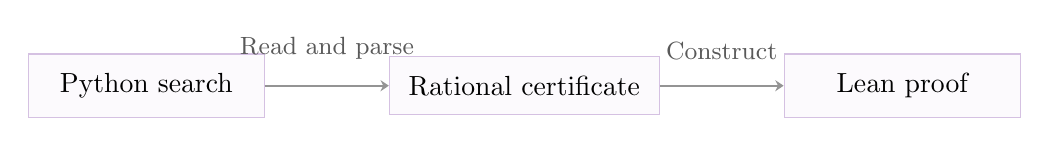
\begin{tikzpicture}[x=1cm,y=1cm]
      \node[proof,minimum width=3cm,align=center] (search) at (-4.8,0) {Python search};
      \node[proof,minimum width=3cm,align=center] (data) at (0,0) {Rational certificate};
      \node[proof,minimum width=3cm,align=center] (prf) at (4.8,0) {Lean proof};
      \draw[flow] (search) -- node[above,labeltext,yshift=6pt]{Read and parse} (data);
      \draw[flow] (data) -- node[above,labeltext,yshift=6pt]{Construct} (prf);
    \end{tikzpicture}
  \end{center}

  \vspace{5mm}
  Each weighted square contributes a nonnegativity proof.

  \vspace{3mm}
  The polynomial identity connects their sum to the original goal.

  \vspace{5mm}
  The kernel checks the completed proof against its claimed type.
  \note{Slide 3 at section 4, after constructing a proof from explicit data.
  Build the string tactic, read a file, print the request, print Python's response,
  then assemble external\_sos. The parser checks format; the constructed
  proof establishes signs and equality. The Python call runs during elaboration.
  Read a saved certificate if setup fails.
  Print axioms of triangle\_external. The solver's numerical correctness is
  not assumed by the resulting proof. Standard real-arithmetic axioms remain.
  Sources: Week 10 adapter, MPiL 7 and 9, LoVe 8's proof-first examples.}
\end{frame}

\section{Proofs by computation}
\begin{frame}{Proofs by reflection}
  To prove a mathematical statement $P(x)$, write an algorithm that checks it.

  \vspace{4mm}
  \textcolor{nyu}{1. Prove once that success implies the statement}
  \[
    \forall x,\qquad \operatorname{check}(x)=\mathrm{true}\;\Longrightarrow\;P(x).
  \]
  This is the algorithm's \textbf{soundness theorem}.

  \vspace{4mm}
  \textcolor{nyu}{2. Run the algorithm on a particular input}
  \[
    \underbrace{\operatorname{check}(x_0)=\mathrm{true}}_{\text{established by computation}}
    \quad\xrightarrow{\ \text{apply the soundness theorem}\ }\quad P(x_0).
  \]

  \note{Slide 4 follows section 5's ordinary monoid proof. Ask for an algorithm
  that recognizes equalities using associativity and identity. Recording factors
  in order suggests flattening. The representation and algorithm are pre-filled;
  the new work is to justify the algorithm and use that theorem.
  In our example success means equality of the two computed lists. This can be
  expressed as a Boolean test, but rfl can also prove the equality directly.
  Returning false is also termination, so the hypothesis is success.
  Source: CPDT, Proof by Reflection, monoid expression simplifier.}
\end{frame}

\begin{frame}{The soundness theorem}
  The algebraic laws justify the normalization algorithm:
  \[
    \underbrace{\operatorname{evalList}_\rho(\operatorname{flatten}(e))}_{\text{interpret the computed list}}
    =\underbrace{\operatorname{eval}_\rho(e)}_{\text{interpret the original expression}}.
  \]

  \vspace{4mm}
  Hence, for every environment $\rho$,
  \[
    \underbrace{\operatorname{flatten}(a)=\operatorname{flatten}(b)}_{\text{equality established by computation}}
    \quad\Longrightarrow\quad
    \underbrace{\operatorname{eval}_\rho(a)=\operatorname{eval}_\rho(b)}_{\text{original mathematical equality}}.
  \]

  \vspace{5mm}
  Applying this theorem reduces our goal to comparing two lists of indices.

  \note{Slide 5 begins section 6. Read flatten\_correct before its supporting lemma.
  Prove the multiplication case and derive reflect\_sound. At 6.3 apply that theorem
  and pause on lhs.flatten = rhs.flatten. Change it to the explicit list equality,
  then use rfl. The values of a, b, c remain arbitrary. The theorem justifies the algorithm using the algebraic laws;
  reduction checks this input. Print reflected.
  Section 7 uses the same equality to explain Decidable and compare evaluation
  methods. Section 8 automates the proof just written.
  Sources: CPDT's monoid simplifier; Timothy Mou's Lean reflection example.}
\end{frame}

\begin{frame}{Decidable propositions}
  A value of \code{Decidable p} contains one of two kinds of evidence:

  \vspace{4mm}
  \begin{center}
  \renewcommand{\arraystretch}{1.7}
  \begin{tabular}{@{}ll@{}}
    \code{isTrue (h : p)} & a proof of $p$ \\
    \code{isFalse (h : $\neg$p)} & a proof that $p$ is false
  \end{tabular}
  \end{center}

  \vspace{4mm}
  The function \code{decide p} returns the corresponding Boolean.
  \pause

  \vspace{4mm}
  \[
    \underbrace{\code{decide p = true}}_{\text{computational evidence}}
    \quad\xrightarrow{\ \code{of\_decide\_eq\_true}\ }\quad p
  \]
  \note{Slide 6 at section 7. Keep the list equality from 6.3 for every computation.
  Inspect Decidable, then run decide on lhs.flatten = rhs.flatten with both
  \#eval and \#reduce. Pause at the bridge theorem. An observed output becomes
  proof evidence when an equality proof is passed to of\_decide\_eq\_true.
  Show lists\_by\_term before the three tactics. The rfl in section 6 already
  proved the list equality directly; decide illustrates the general decision
  procedure interface. Sources: TPiL Decidable; FPiL Standard Classes.}
\end{frame}

\begin{frame}{Where does the computation run?}
  \renewcommand{\arraystretch}{1.45}
  \setlength{\tabcolsep}{5pt}
  \begin{tabular}{@{}>{\raggedright\arraybackslash}p{3cm}>{\raggedright\arraybackslash}p{6cm}>{\raggedright\arraybackslash}p{5.2cm}@{}}
    \textcolor{nyu}{Tactic} & \textcolor{nyu}{Computation} & \textcolor{nyu}{Evidence checked by the kernel} \\
    \code{decide} & Reduce during elaboration; the kernel checks the computational proof. & A proof using definitional equality. \\[2mm]
    \code{decide +kernel} & Validate the computational proof directly in the kernel. & A proof using definitional equality. \\[2mm]
    \code{native\_decide} & Evaluate compiled code and record its result as an axiom. & A proof depending on that additional axiom.
  \end{tabular}

  \vspace{5mm}
  \code{\#print axioms} exposes the dependencies of the finished theorem.

  \vspace{3mm}
  Native computation extends trust to the compiler and execution machinery.
  \note{Slide 7 at 7.2. Compare the identical list equality with each method.
  On v4.34.0-rc2, ordinary decide first reduces during elaboration, then submits
  a computational proof for kernel checking. The +kernel path validates an
  auxiliary lemma directly in the kernel. native\_decide executes compiled code
  and introduces a fresh axiom asserting the result. Print its actual name.
  In 7.3 replace lists\_native by lists\_kernel and inspect the finished theorem's
  dependencies. This changes how its computational premise is justified while
  retaining the same soundness theorem. The small example illustrates evidence,
  not performance. Recall Week 6's finite checks for the motivation to compute
  efficiently. Sources: pinned Decide.lean and Native.lean.}
\end{frame}

\end{document}
